\documentclass[../main.tex]{subfiles}

Kommen wir nun zum Herzstück der Seminararbeit: Das Infrarotspektrometer. Es handelt sich um ein Werkzeug der Spektroskopie, das mithilfe der Absorptionseigenschaften der Elemente am Infrarotlicht eigenschaften von Substanzen nachweist.

\subsection{Komponenten}

\begin{figure}[ht]
    \centering
    \begin{subfigure}[b]{0.25\textwidth}
        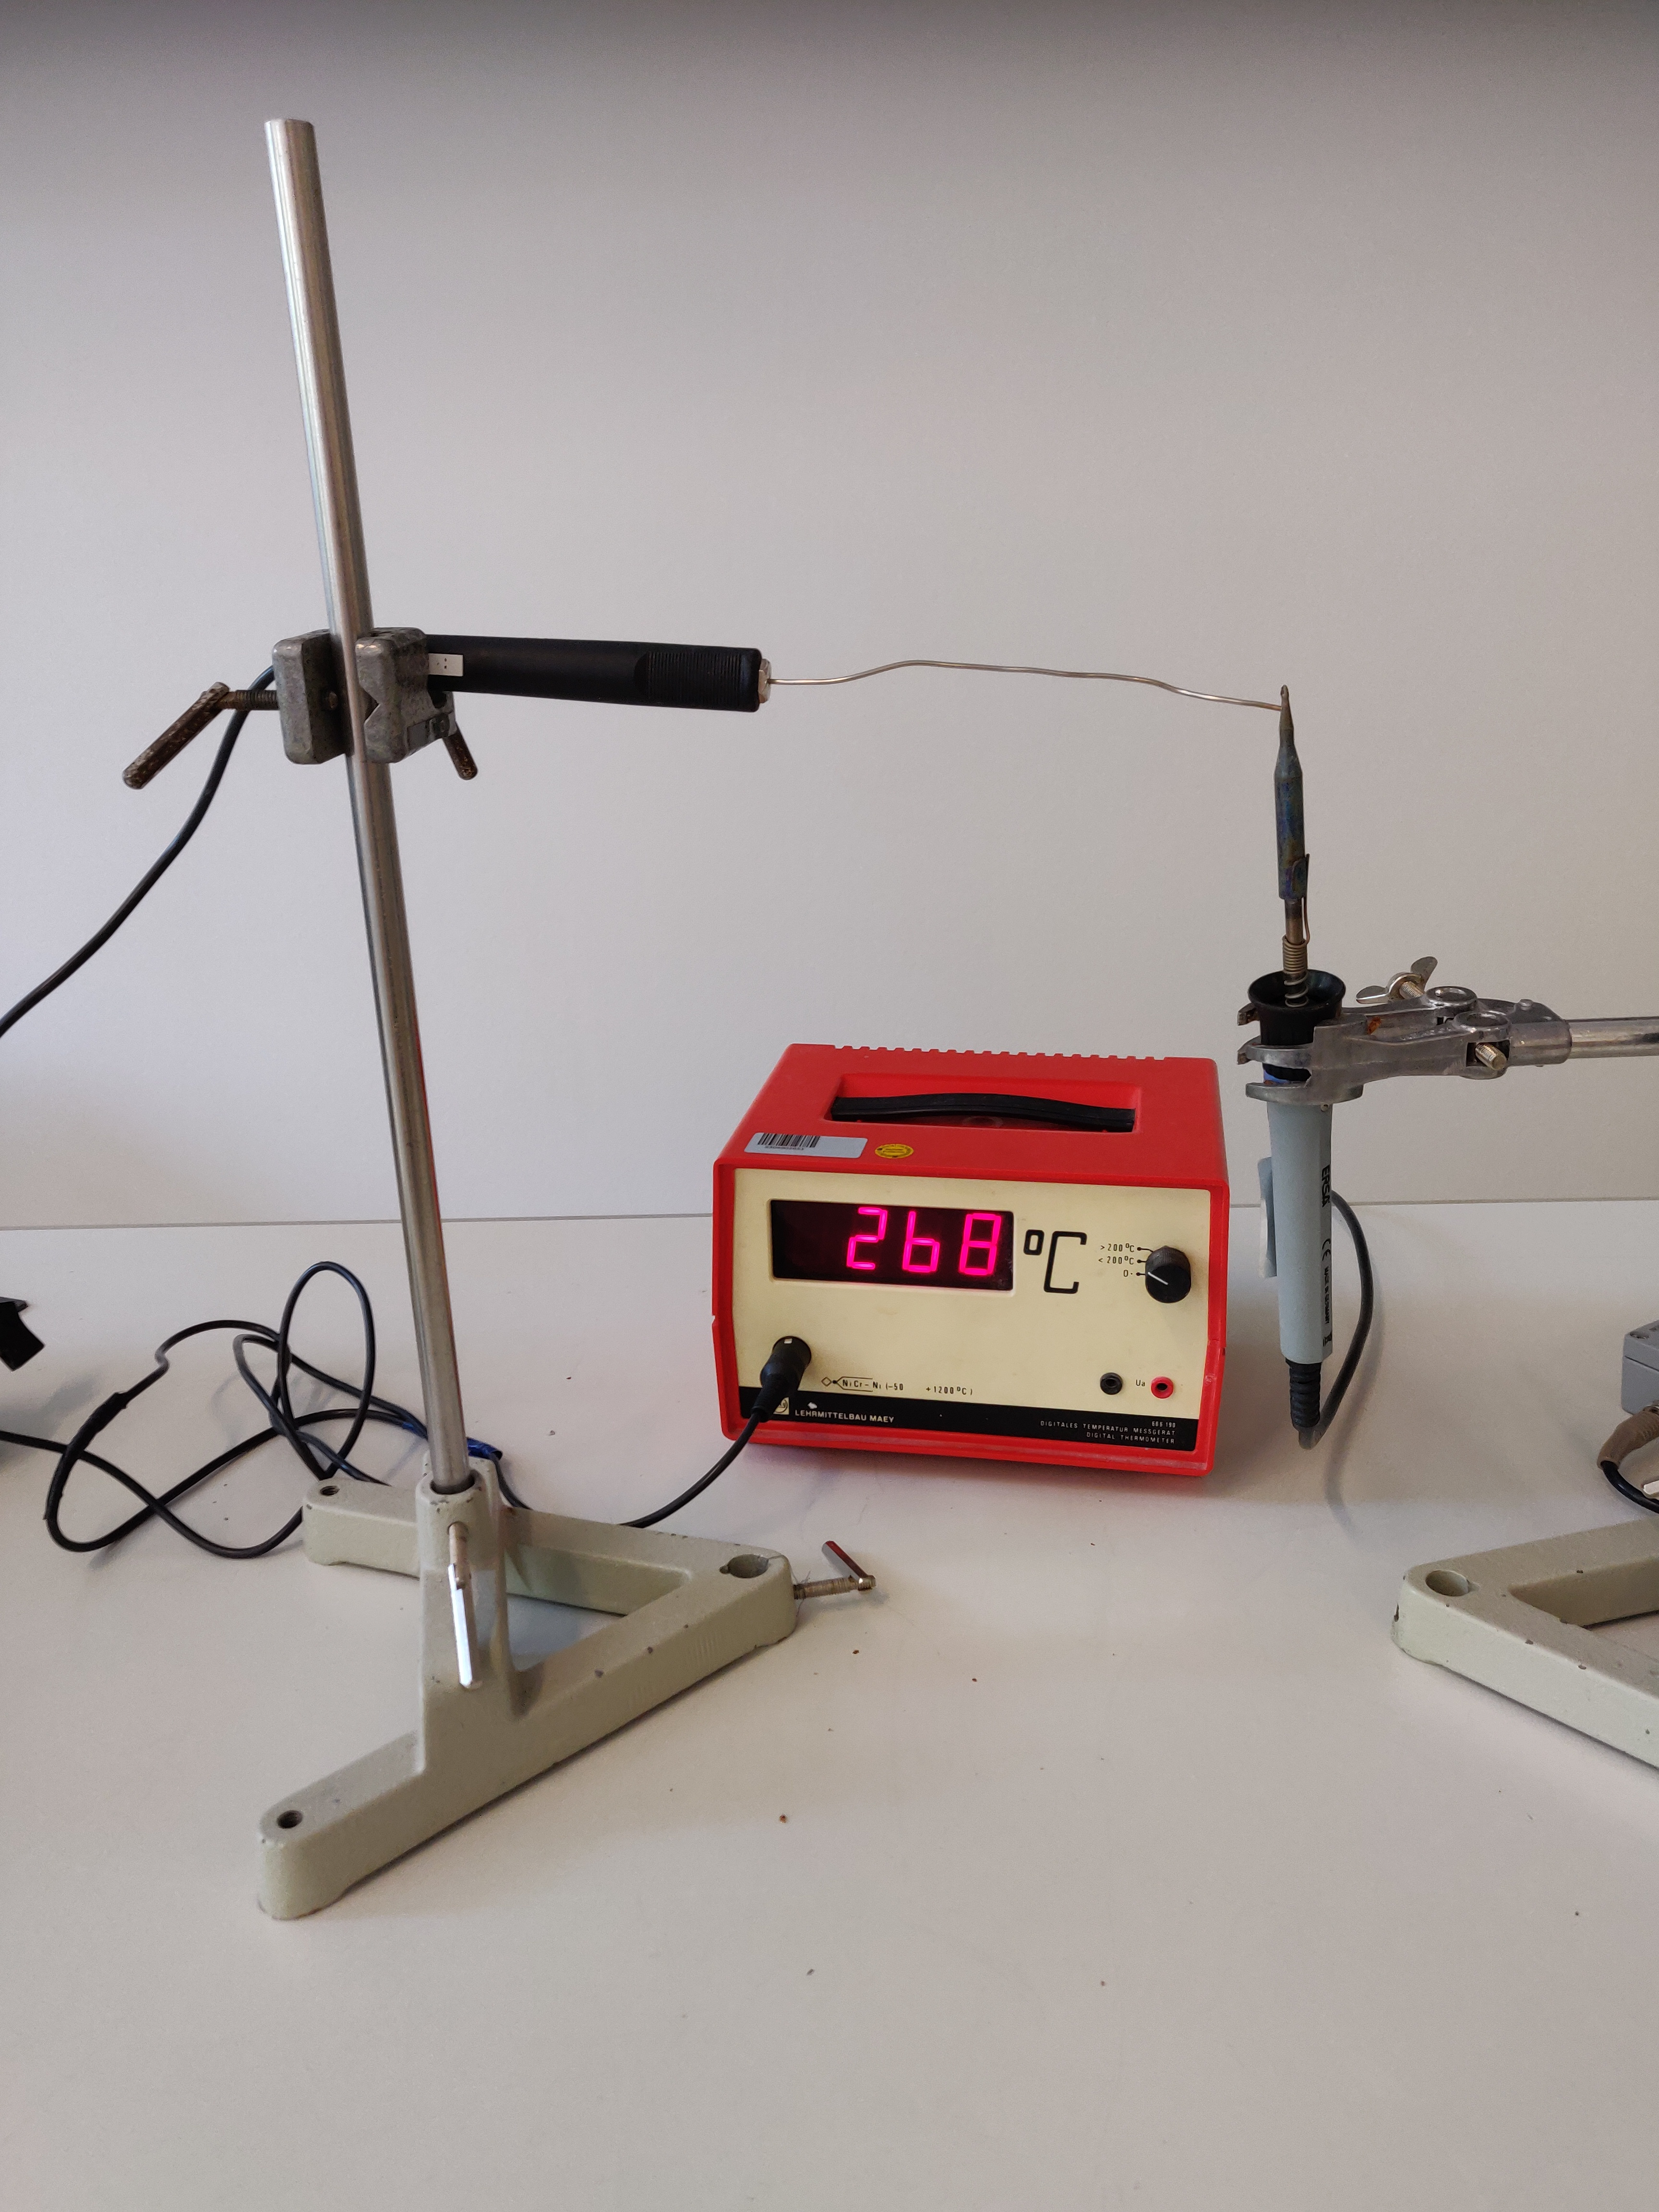
\includegraphics[width=\textwidth]{experiment/11-loetkolben-temperatur.jpg}
        \caption{Lötkolben}
        \label{fig:loetkolben}
    \end{subfigure}
    \begin{subfigure}[b]{0.25\textwidth}
        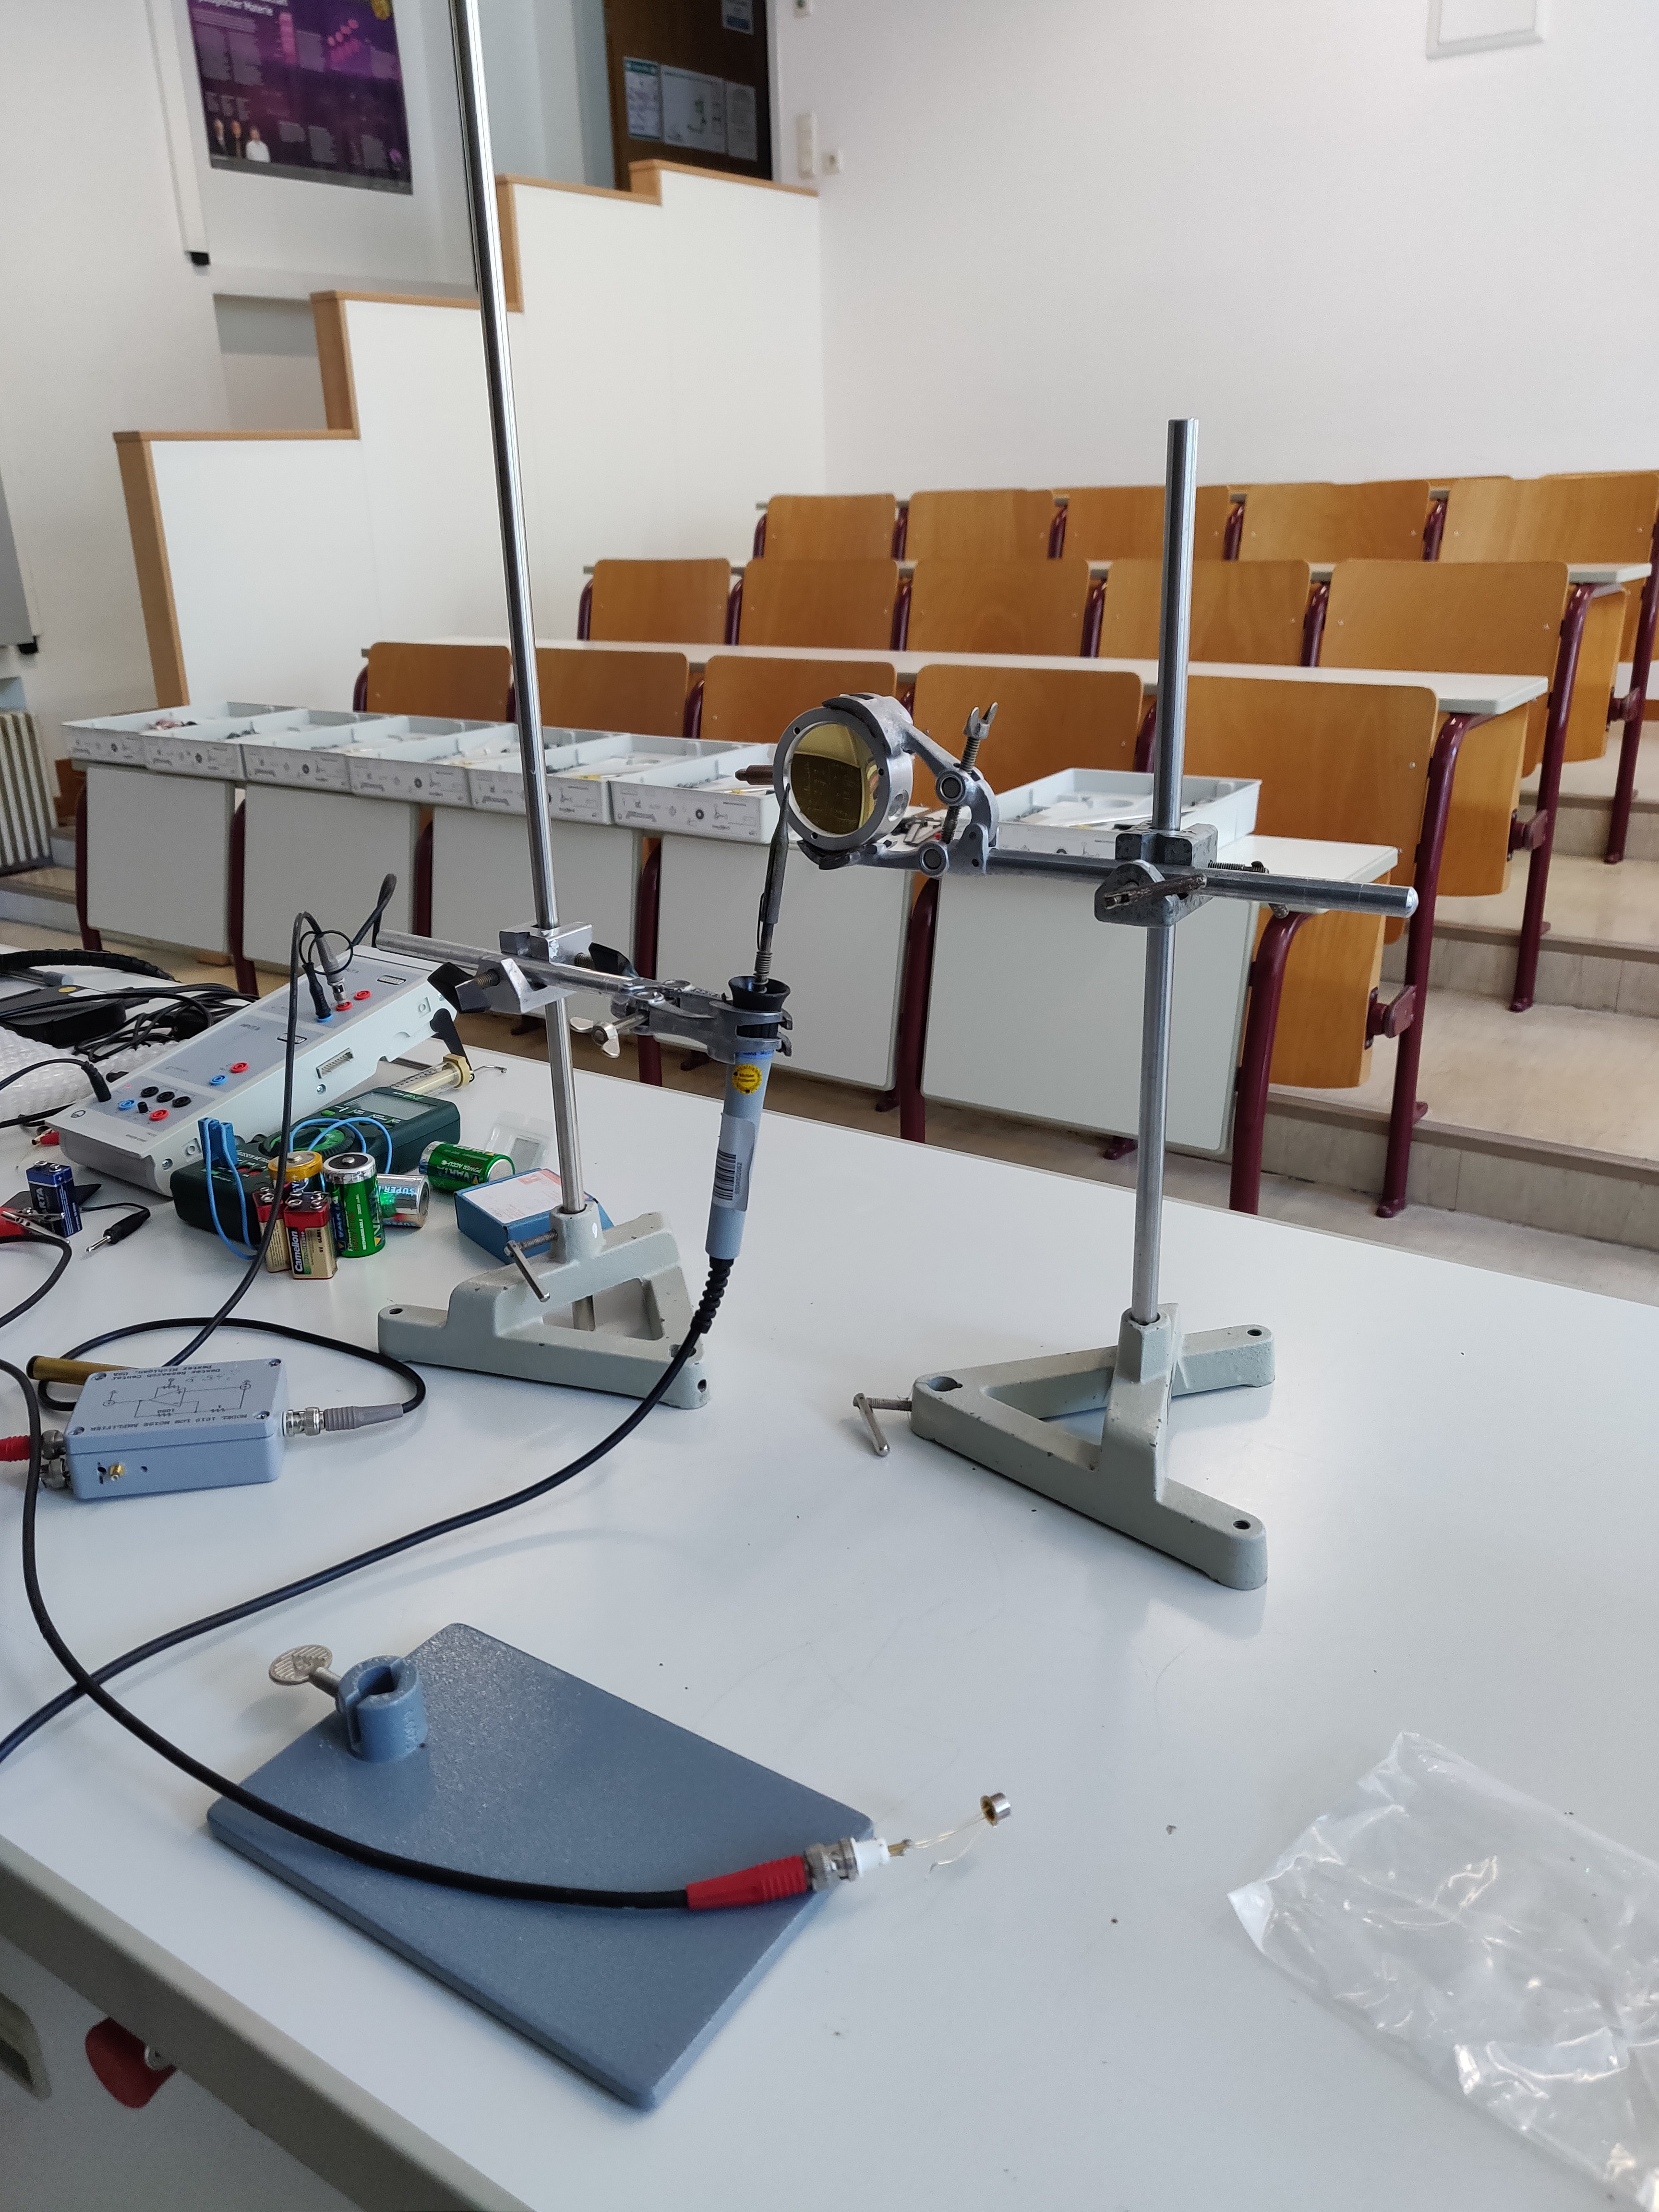
\includegraphics[width=\textwidth]{experiment/13-loetkolben-spiegel.jpg}
        \caption{Lötkolben mit Spiegel}
        \label{fig:loetkolben_mit_spiegel}
    \end{subfigure}
    \begin{subfigure}[b]{0.25\textwidth}
        \includegraphics[width=\textwidth]{experiment/29-leypold-gitter.jpg}
        \caption{Leypold Gitter}
        \label{fig:gitter_600l}
    \end{subfigure}
    \caption{Diverse Komponenten}
\end{figure}

\subsubsection{Strahlquelle}
Zunächst benötigen wir eine Infrarot-Strahlquelle, welche die Substanz durchdringt und danach mit einem Detektor gemessen wird. Als Strahlquelle bietet sich ein Lötkolben an (Abb. \ref{fig:loetkolben}).


% λ × T = b
% Lötkolben

\subsubsection{Abbildende Optik}
Um die Strahlung unseres Lötkolbens in eine Richtung zu fokusieren, müssen die nach außen gerichteten Wellen reflektiert werden. Ein Parabelförmiger Spiegel reflektiert die Strahlung so, dass sie in eine Richtung zeigt (Abb. \ref{fig:loetkolben_mit_spiegel}).

% Spiegel

\subsubsection{Optisches Gitter}
Das Gitter beugt die Strahlung in die verschiedenen Wellenlängen. Hierfür gibt es Gitter verschiedener Dichten, oder auch Reflexionsgitter, welche sowohl beugen als auch reflektieren (Abb. \ref{fig:gitter_600l}).
Folgende Formel beschreibt die position der Maxima (vielfache von $\lambda$) auf Basis der Gitterdichte $b$. 
\[
    k \lambda = b \sin{\alpha}
\]



% 600 Linien / mm
% Leypold
% Reflexionsgitter
